% Options for packages loaded elsewhere
\PassOptionsToPackage{unicode}{hyperref}
\PassOptionsToPackage{hyphens}{url}
%
\documentclass[
  10pt,
  ignorenonframetext,
  aspectratio=1612]{beamer}
\usepackage{pgfpages}
\setbeamertemplate{caption}[numbered]
\setbeamertemplate{caption label separator}{: }
\setbeamercolor{caption name}{fg=normal text.fg}
\beamertemplatenavigationsymbolsempty
% Prevent slide breaks in the middle of a paragraph
\widowpenalties 1 10000
\raggedbottom
\setbeamertemplate{part page}{
  \centering
  \begin{beamercolorbox}[sep=16pt,center]{part title}
    \usebeamerfont{part title}\insertpart\par
  \end{beamercolorbox}
}
\setbeamertemplate{section page}{
  \centering
  \begin{beamercolorbox}[sep=12pt,center]{part title}
    \usebeamerfont{section title}\insertsection\par
  \end{beamercolorbox}
}
\setbeamertemplate{subsection page}{
  \centering
  \begin{beamercolorbox}[sep=8pt,center]{part title}
    \usebeamerfont{subsection title}\insertsubsection\par
  \end{beamercolorbox}
}
\AtBeginPart{
  \frame{\partpage}
}
\AtBeginSection{
  \ifbibliography
  \else
    \frame{\sectionpage}
  \fi
}
\AtBeginSubsection{
  \frame{\subsectionpage}
}
\usepackage{amsmath,amssymb}
\usepackage{iftex}
\ifPDFTeX
  \usepackage[T1]{fontenc}
  \usepackage[utf8]{inputenc}
  \usepackage{textcomp} % provide euro and other symbols
\else % if luatex or xetex
  \usepackage{unicode-math} % this also loads fontspec
  \defaultfontfeatures{Scale=MatchLowercase}
  \defaultfontfeatures[\rmfamily]{Ligatures=TeX,Scale=1}
\fi
\usepackage{lmodern}
\usetheme[]{Warsaw}
\ifPDFTeX\else
  % xetex/luatex font selection
\fi
% Use upquote if available, for straight quotes in verbatim environments
\IfFileExists{upquote.sty}{\usepackage{upquote}}{}
\IfFileExists{microtype.sty}{% use microtype if available
  \usepackage[]{microtype}
  \UseMicrotypeSet[protrusion]{basicmath} % disable protrusion for tt fonts
}{}
\makeatletter
\@ifundefined{KOMAClassName}{% if non-KOMA class
  \IfFileExists{parskip.sty}{%
    \usepackage{parskip}
  }{% else
    \setlength{\parindent}{0pt}
    \setlength{\parskip}{6pt plus 2pt minus 1pt}}
}{% if KOMA class
  \KOMAoptions{parskip=half}}
\makeatother
\usepackage{xcolor}
\newif\ifbibliography
\usepackage{color}
\usepackage{fancyvrb}
\newcommand{\VerbBar}{|}
\newcommand{\VERB}{\Verb[commandchars=\\\{\}]}
\DefineVerbatimEnvironment{Highlighting}{Verbatim}{commandchars=\\\{\}}
% Add ',fontsize=\small' for more characters per line
\usepackage{framed}
\definecolor{shadecolor}{RGB}{248,248,248}
\newenvironment{Shaded}{\begin{snugshade}}{\end{snugshade}}
\newcommand{\AlertTok}[1]{\textcolor[rgb]{0.94,0.16,0.16}{#1}}
\newcommand{\AnnotationTok}[1]{\textcolor[rgb]{0.56,0.35,0.01}{\textbf{\textit{#1}}}}
\newcommand{\AttributeTok}[1]{\textcolor[rgb]{0.13,0.29,0.53}{#1}}
\newcommand{\BaseNTok}[1]{\textcolor[rgb]{0.00,0.00,0.81}{#1}}
\newcommand{\BuiltInTok}[1]{#1}
\newcommand{\CharTok}[1]{\textcolor[rgb]{0.31,0.60,0.02}{#1}}
\newcommand{\CommentTok}[1]{\textcolor[rgb]{0.56,0.35,0.01}{\textit{#1}}}
\newcommand{\CommentVarTok}[1]{\textcolor[rgb]{0.56,0.35,0.01}{\textbf{\textit{#1}}}}
\newcommand{\ConstantTok}[1]{\textcolor[rgb]{0.56,0.35,0.01}{#1}}
\newcommand{\ControlFlowTok}[1]{\textcolor[rgb]{0.13,0.29,0.53}{\textbf{#1}}}
\newcommand{\DataTypeTok}[1]{\textcolor[rgb]{0.13,0.29,0.53}{#1}}
\newcommand{\DecValTok}[1]{\textcolor[rgb]{0.00,0.00,0.81}{#1}}
\newcommand{\DocumentationTok}[1]{\textcolor[rgb]{0.56,0.35,0.01}{\textbf{\textit{#1}}}}
\newcommand{\ErrorTok}[1]{\textcolor[rgb]{0.64,0.00,0.00}{\textbf{#1}}}
\newcommand{\ExtensionTok}[1]{#1}
\newcommand{\FloatTok}[1]{\textcolor[rgb]{0.00,0.00,0.81}{#1}}
\newcommand{\FunctionTok}[1]{\textcolor[rgb]{0.13,0.29,0.53}{\textbf{#1}}}
\newcommand{\ImportTok}[1]{#1}
\newcommand{\InformationTok}[1]{\textcolor[rgb]{0.56,0.35,0.01}{\textbf{\textit{#1}}}}
\newcommand{\KeywordTok}[1]{\textcolor[rgb]{0.13,0.29,0.53}{\textbf{#1}}}
\newcommand{\NormalTok}[1]{#1}
\newcommand{\OperatorTok}[1]{\textcolor[rgb]{0.81,0.36,0.00}{\textbf{#1}}}
\newcommand{\OtherTok}[1]{\textcolor[rgb]{0.56,0.35,0.01}{#1}}
\newcommand{\PreprocessorTok}[1]{\textcolor[rgb]{0.56,0.35,0.01}{\textit{#1}}}
\newcommand{\RegionMarkerTok}[1]{#1}
\newcommand{\SpecialCharTok}[1]{\textcolor[rgb]{0.81,0.36,0.00}{\textbf{#1}}}
\newcommand{\SpecialStringTok}[1]{\textcolor[rgb]{0.31,0.60,0.02}{#1}}
\newcommand{\StringTok}[1]{\textcolor[rgb]{0.31,0.60,0.02}{#1}}
\newcommand{\VariableTok}[1]{\textcolor[rgb]{0.00,0.00,0.00}{#1}}
\newcommand{\VerbatimStringTok}[1]{\textcolor[rgb]{0.31,0.60,0.02}{#1}}
\newcommand{\WarningTok}[1]{\textcolor[rgb]{0.56,0.35,0.01}{\textbf{\textit{#1}}}}
\usepackage{graphicx}
\makeatletter
\def\maxwidth{\ifdim\Gin@nat@width>\linewidth\linewidth\else\Gin@nat@width\fi}
\def\maxheight{\ifdim\Gin@nat@height>\textheight\textheight\else\Gin@nat@height\fi}
\makeatother
% Scale images if necessary, so that they will not overflow the page
% margins by default, and it is still possible to overwrite the defaults
% using explicit options in \includegraphics[width, height, ...]{}
\setkeys{Gin}{width=\maxwidth,height=\maxheight,keepaspectratio}
% Set default figure placement to htbp
\makeatletter
\def\fps@figure{htbp}
\makeatother
\setlength{\emergencystretch}{3em} % prevent overfull lines
\providecommand{\tightlist}{%
  \setlength{\itemsep}{0pt}\setlength{\parskip}{0pt}}
\setcounter{secnumdepth}{-\maxdimen} % remove section numbering
\ifLuaTeX
  \usepackage{selnolig}  % disable illegal ligatures
\fi
\usepackage{bookmark}
\IfFileExists{xurl.sty}{\usepackage{xurl}}{} % add URL line breaks if available
\urlstyle{same}
\hypersetup{
  pdftitle={Análisis Descriptivo De la Serie de Tiempo del Café},
  pdfauthor={Angel Granados, Wilson Jerez, Santiago Montejo},
  hidelinks,
  pdfcreator={LaTeX via pandoc}}

\title{Análisis Descriptivo De la Serie de Tiempo del Café}
\author{Angel Granados, Wilson Jerez, Santiago Montejo}
\date{Junio 2024}

\begin{document}
\frame{\titlepage}

\begin{frame}{Introducción}
\phantomsection\label{introducciuxf3n}
El presente informe tiene como objetivo analizar y visualizar los
precios del café a lo largo del tiempo. Se utilizarán técnicas de
análisis descriptivo para explorar las tendencias y patrones en los
datos.
\end{frame}

\begin{frame}[fragile]{Carga de bibliotecas y datos}
\phantomsection\label{carga-de-bibliotecas-y-datos}
\begin{Shaded}
\begin{Highlighting}[]
\FunctionTok{library}\NormalTok{(ggplot2)}
\FunctionTok{library}\NormalTok{(urca)}

\FunctionTok{setwd}\NormalTok{(}\StringTok{"\textasciitilde{}/Documentos/Cafe"}\NormalTok{) }\CommentTok{\# Establecer ruta de trabajo}
\NormalTok{datosHist }\OtherTok{\textless{}{-}} \FunctionTok{read.csv}\NormalTok{(}\StringTok{\textquotesingle{}datosHist.csv\textquotesingle{}}\NormalTok{)}
\NormalTok{datosHist}\SpecialCharTok{$}\NormalTok{Fecha }\OtherTok{\textless{}{-}} \FunctionTok{as.Date}\NormalTok{(datosHist}\SpecialCharTok{$}\NormalTok{Fecha)}
\end{Highlighting}
\end{Shaded}
\end{frame}

\begin{frame}[fragile]{Serie de tiempo de todos los datos}
\phantomsection\label{serie-de-tiempo-de-todos-los-datos}
\begin{Shaded}
\begin{Highlighting}[]
\NormalTok{KCN4 }\OtherTok{\textless{}{-}} \FunctionTok{ts}\NormalTok{(datosHist}\SpecialCharTok{$}\NormalTok{precio\_promedio,}\AttributeTok{freq=}\DecValTok{12}\NormalTok{)}
\FunctionTok{plot}\NormalTok{(datosHist}\SpecialCharTok{$}\NormalTok{Fecha, KCN4, }\AttributeTok{type =} \StringTok{"l"}\NormalTok{, }\AttributeTok{xlab =} \StringTok{"Fecha"}\NormalTok{, }
     \AttributeTok{ylab =} \StringTok{"Precio Promedio"}\NormalTok{, }\AttributeTok{main =} \StringTok{"Precios del Café"}\NormalTok{)}
\end{Highlighting}
\end{Shaded}

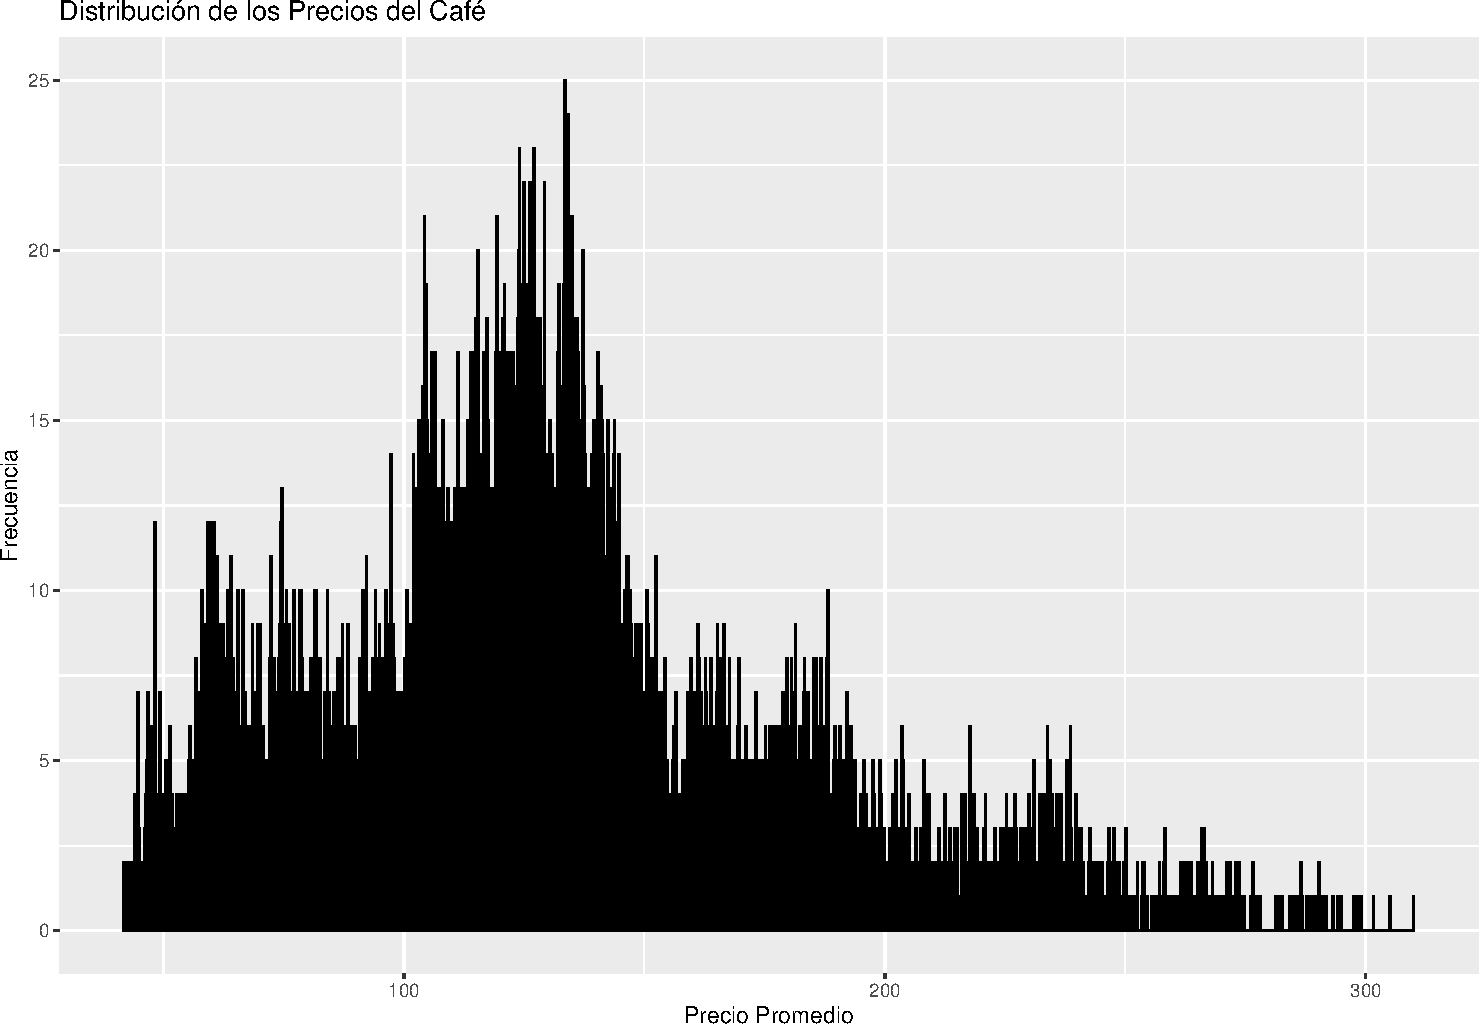
\includegraphics{Informe_files/figure-beamer/unnamed-chunk-2-1.pdf}
\end{frame}

\begin{frame}[fragile]{Serie de tiempo por año}
\phantomsection\label{serie-de-tiempo-por-auxf1o}
\begin{Shaded}
\begin{Highlighting}[]
\CommentTok{\# Crear un bucle for para particionar los datos por año}
\ControlFlowTok{for}\NormalTok{ (i }\ControlFlowTok{in} \DecValTok{1980}\SpecialCharTok{:}\DecValTok{2023}\NormalTok{) \{}
\NormalTok{  start\_date }\OtherTok{\textless{}{-}} \FunctionTok{as.Date}\NormalTok{(}\FunctionTok{paste}\NormalTok{(i, }\StringTok{"{-}01{-}01"}\NormalTok{, }\AttributeTok{sep =} \StringTok{""}\NormalTok{))}
\NormalTok{  end\_date }\OtherTok{\textless{}{-}} \FunctionTok{as.Date}\NormalTok{(}\FunctionTok{paste}\NormalTok{(i }\SpecialCharTok{+} \DecValTok{1}\NormalTok{, }\StringTok{"{-}01{-}01"}\NormalTok{, }\AttributeTok{sep =} \StringTok{""}\NormalTok{))}
  
\NormalTok{  datosporAño }\OtherTok{\textless{}{-}} \FunctionTok{subset}\NormalTok{(datosHist, }
\NormalTok{                        Fecha }\SpecialCharTok{\textgreater{}=}\NormalTok{ start\_date }
                        \SpecialCharTok{\&}\NormalTok{ Fecha }\SpecialCharTok{\textless{}}\NormalTok{ end\_date)}
\NormalTok{  KCN4porAño }\OtherTok{\textless{}{-}} \FunctionTok{ts}\NormalTok{(datosporAño}\SpecialCharTok{$}\NormalTok{precio\_promedio, }
                   \AttributeTok{frequency =} \DecValTok{12}\NormalTok{)}
  \FunctionTok{assign}\NormalTok{(}\FunctionTok{paste0}\NormalTok{(}\StringTok{"Datos\_Hist\_"}\NormalTok{, i), datosporAño)}
  \FunctionTok{assign}\NormalTok{(}\FunctionTok{paste0}\NormalTok{(}\StringTok{"KCN4\_"}\NormalTok{, i), KCN4porAño)}
\NormalTok{\}}
\end{Highlighting}
\end{Shaded}
\end{frame}

\begin{frame}[fragile]{}
\phantomsection\label{section}
\begin{Shaded}
\begin{Highlighting}[]
\FunctionTok{plot}\NormalTok{(Datos\_Hist\_2000}\SpecialCharTok{$}\NormalTok{Fecha, KCN4\_2000, }\AttributeTok{type =} \StringTok{"l"}\NormalTok{, }
     \AttributeTok{xlab =} \StringTok{"Fecha"}\NormalTok{, }
     \AttributeTok{ylab =} \StringTok{"Precio Promedio"}\NormalTok{, }\AttributeTok{main =} \StringTok{"Precios del Café"}\NormalTok{)}
\end{Highlighting}
\end{Shaded}

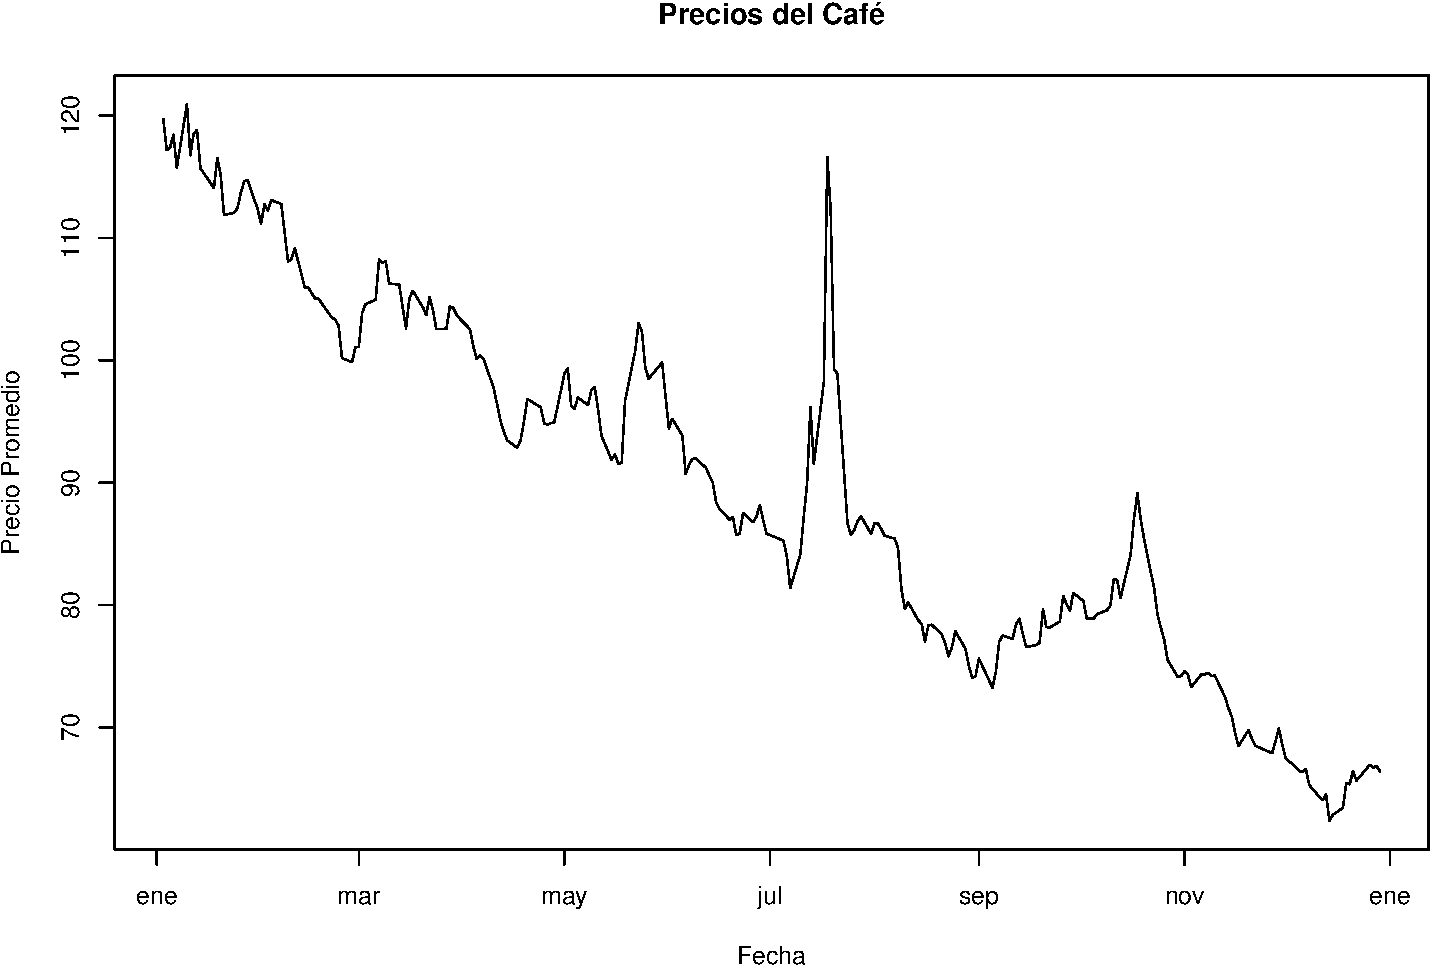
\includegraphics{Informe_files/figure-beamer/unnamed-chunk-4-1.pdf}
\end{frame}

\begin{frame}[fragile]{Cálculo de la variación de las series de tiempo}
\phantomsection\label{cuxe1lculo-de-la-variaciuxf3n-de-las-series-de-tiempo}
\begin{Shaded}
\begin{Highlighting}[]
\FunctionTok{plot}\NormalTok{(}\FunctionTok{diff}\NormalTok{(}\FunctionTok{log}\NormalTok{(KCN4))) }
\FunctionTok{abline}\NormalTok{(}\AttributeTok{h=}\DecValTok{0}\NormalTok{)}
\end{Highlighting}
\end{Shaded}

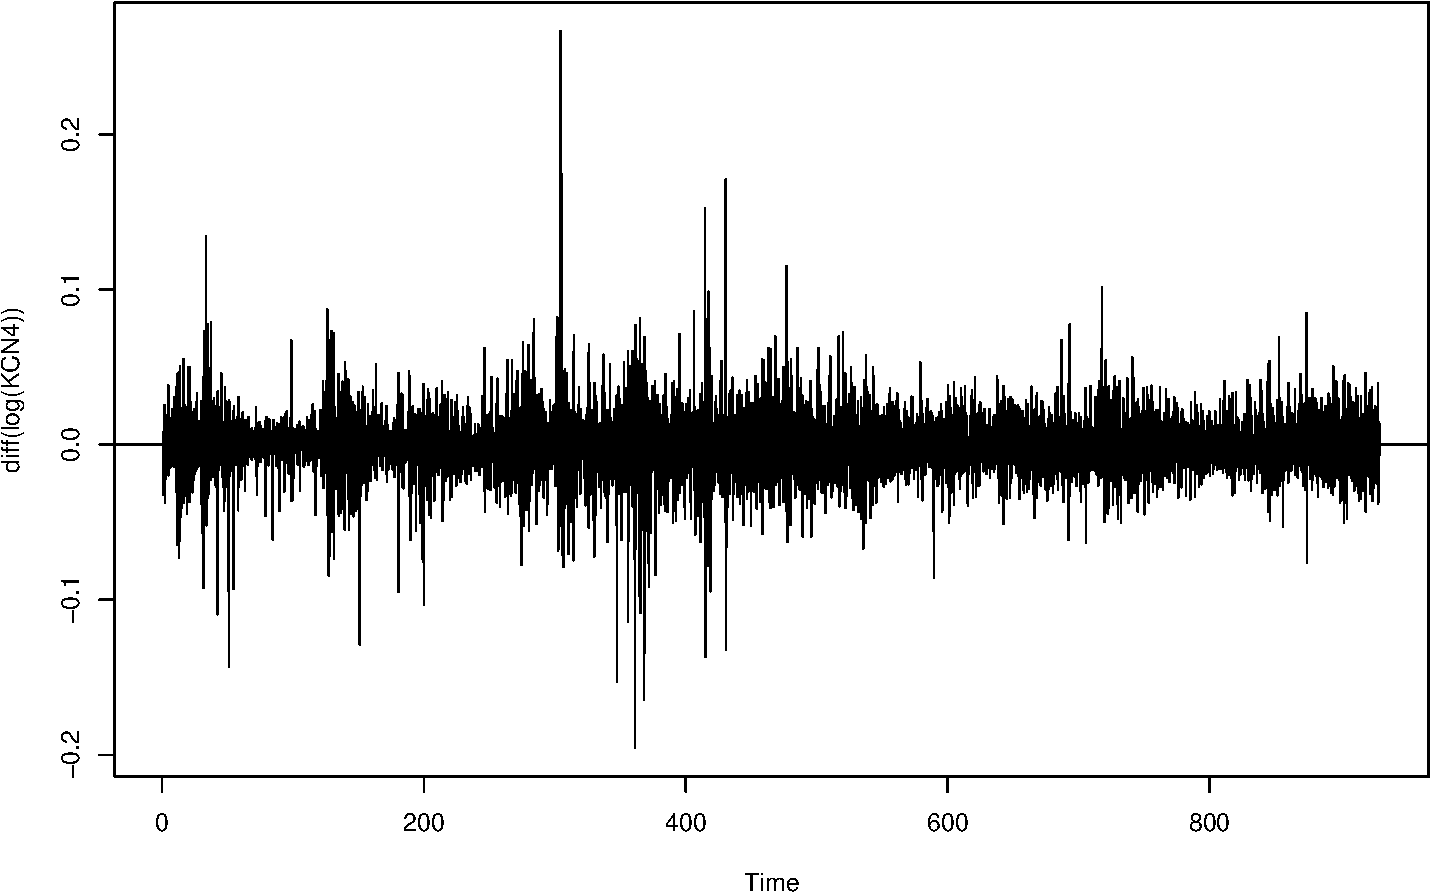
\includegraphics{Informe_files/figure-beamer/unnamed-chunk-5-1.pdf}
\end{frame}

\begin{frame}[fragile]{}
\phantomsection\label{section-1}
\begin{Shaded}
\begin{Highlighting}[]
\FunctionTok{plot}\NormalTok{(}\FunctionTok{diff}\NormalTok{(}\FunctionTok{log}\NormalTok{(KCN4\_2000))) }
\FunctionTok{abline}\NormalTok{(}\AttributeTok{h=}\DecValTok{0}\NormalTok{)}
\end{Highlighting}
\end{Shaded}

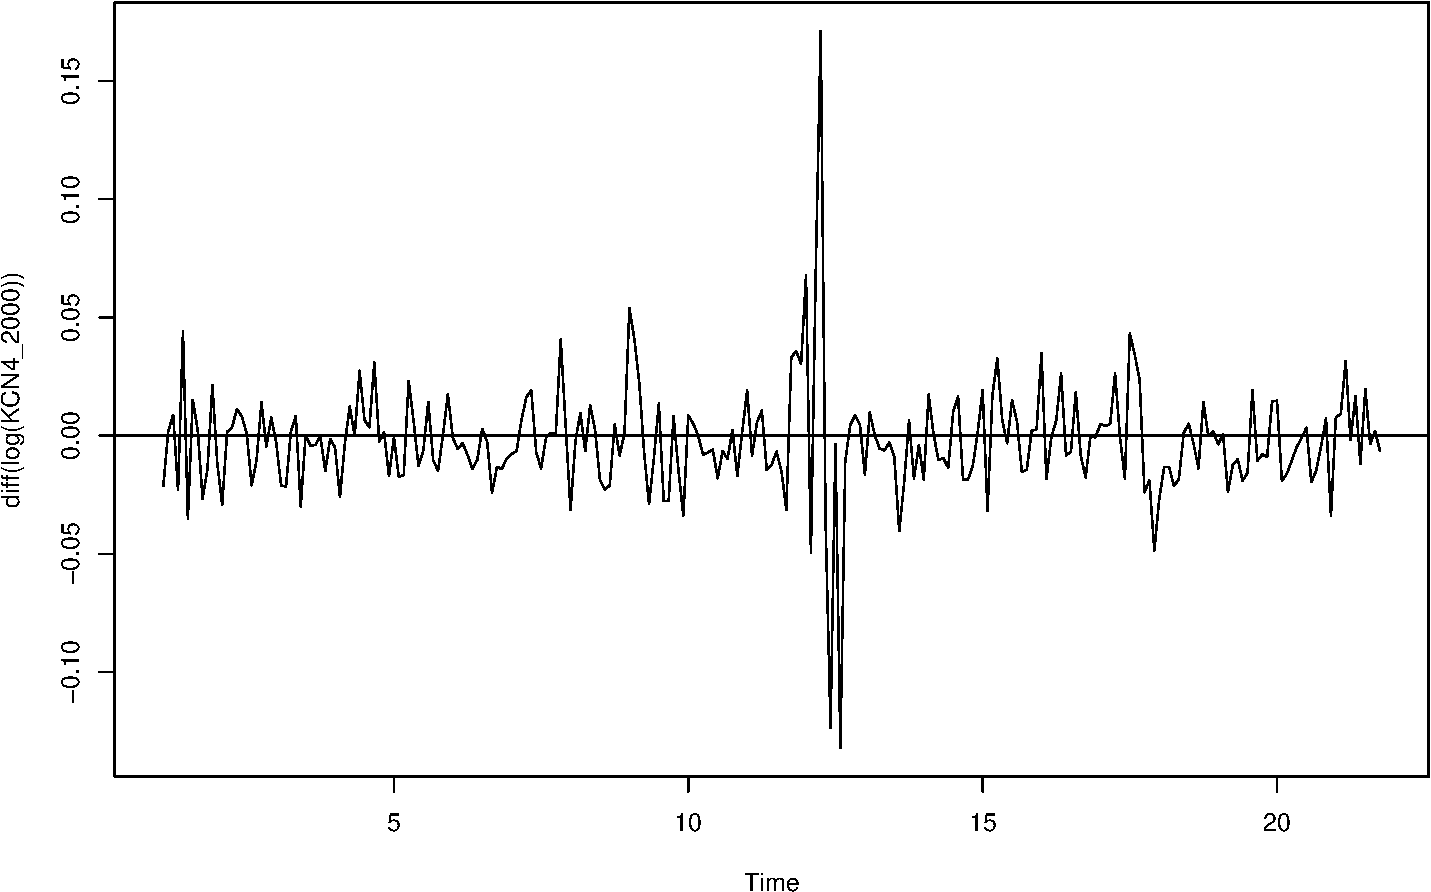
\includegraphics{Informe_files/figure-beamer/unnamed-chunk-6-1.pdf}
\end{frame}

\begin{frame}[fragile]{Descomposición de la serie de tiempo}
\phantomsection\label{descomposiciuxf3n-de-la-serie-de-tiempo}
\begin{Shaded}
\begin{Highlighting}[]
\NormalTok{decomposition\_2000 }\OtherTok{\textless{}{-}} \FunctionTok{decompose}\NormalTok{(KCN4\_2000, }
                                \AttributeTok{type =} \StringTok{"additive"}\NormalTok{)}
\FunctionTok{plot}\NormalTok{(decomposition\_2000}\SpecialCharTok{$}\NormalTok{x, }
     \AttributeTok{ylab =} \StringTok{"Serie de Tiempo Original"}\NormalTok{, }\AttributeTok{xlab =} \StringTok{""}\NormalTok{)}
\end{Highlighting}
\end{Shaded}

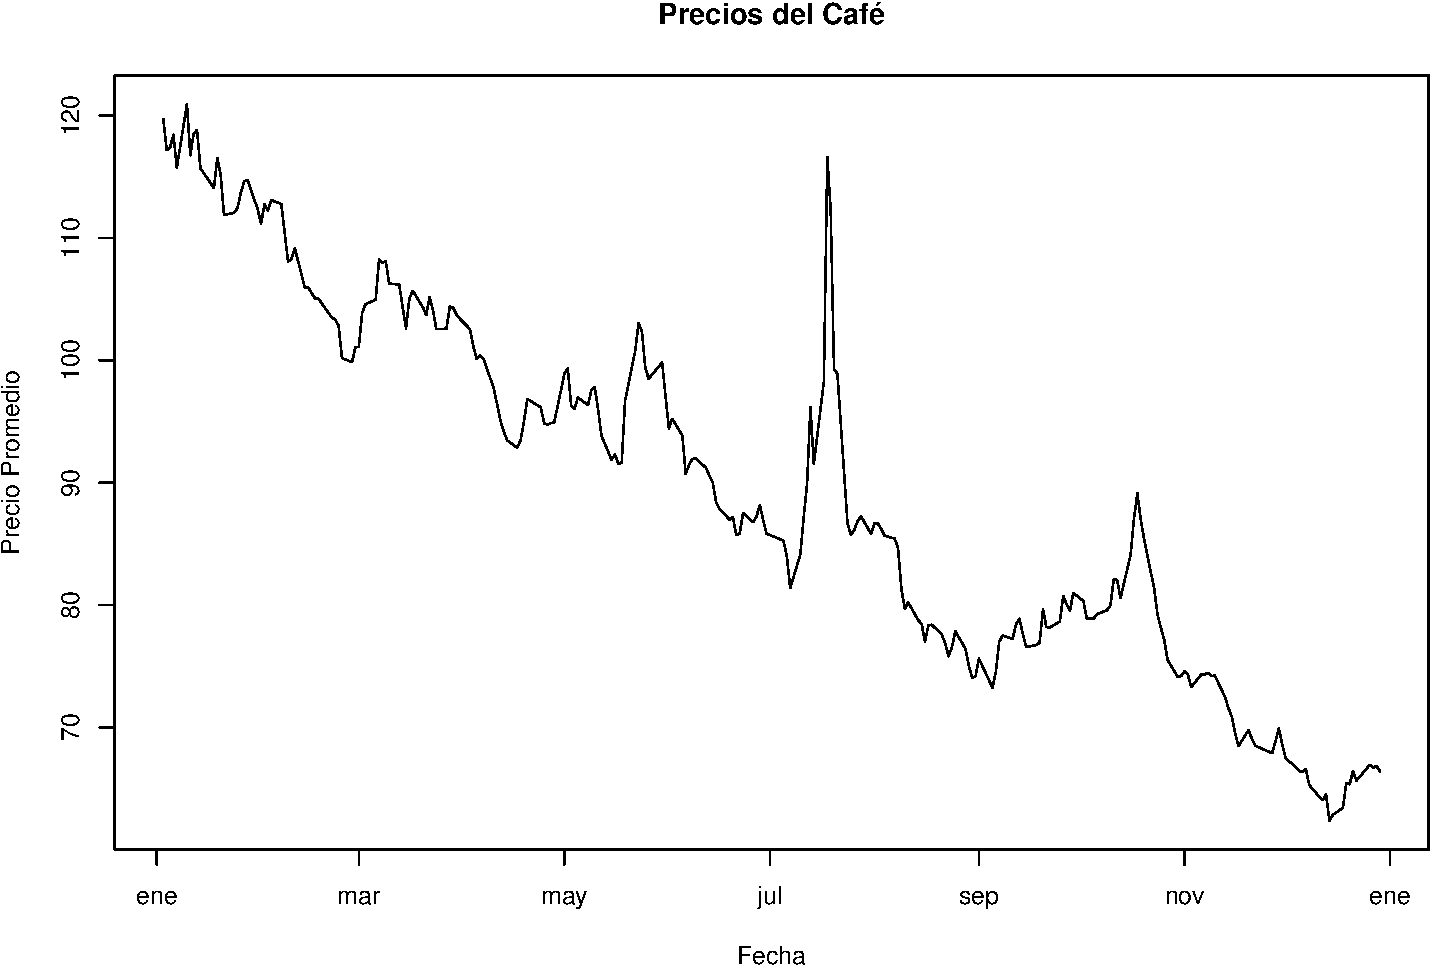
\includegraphics{Informe_files/figure-beamer/unnamed-chunk-7-1.pdf}
\end{frame}

\begin{frame}[fragile]{}
\phantomsection\label{section-2}
\begin{Shaded}
\begin{Highlighting}[]
\FunctionTok{plot}\NormalTok{(decomposition\_2000}\SpecialCharTok{$}\NormalTok{trend, }
     \AttributeTok{ylab =} \StringTok{"Tendencia"}\NormalTok{, }\AttributeTok{xlab =} \StringTok{""}\NormalTok{)}
\end{Highlighting}
\end{Shaded}

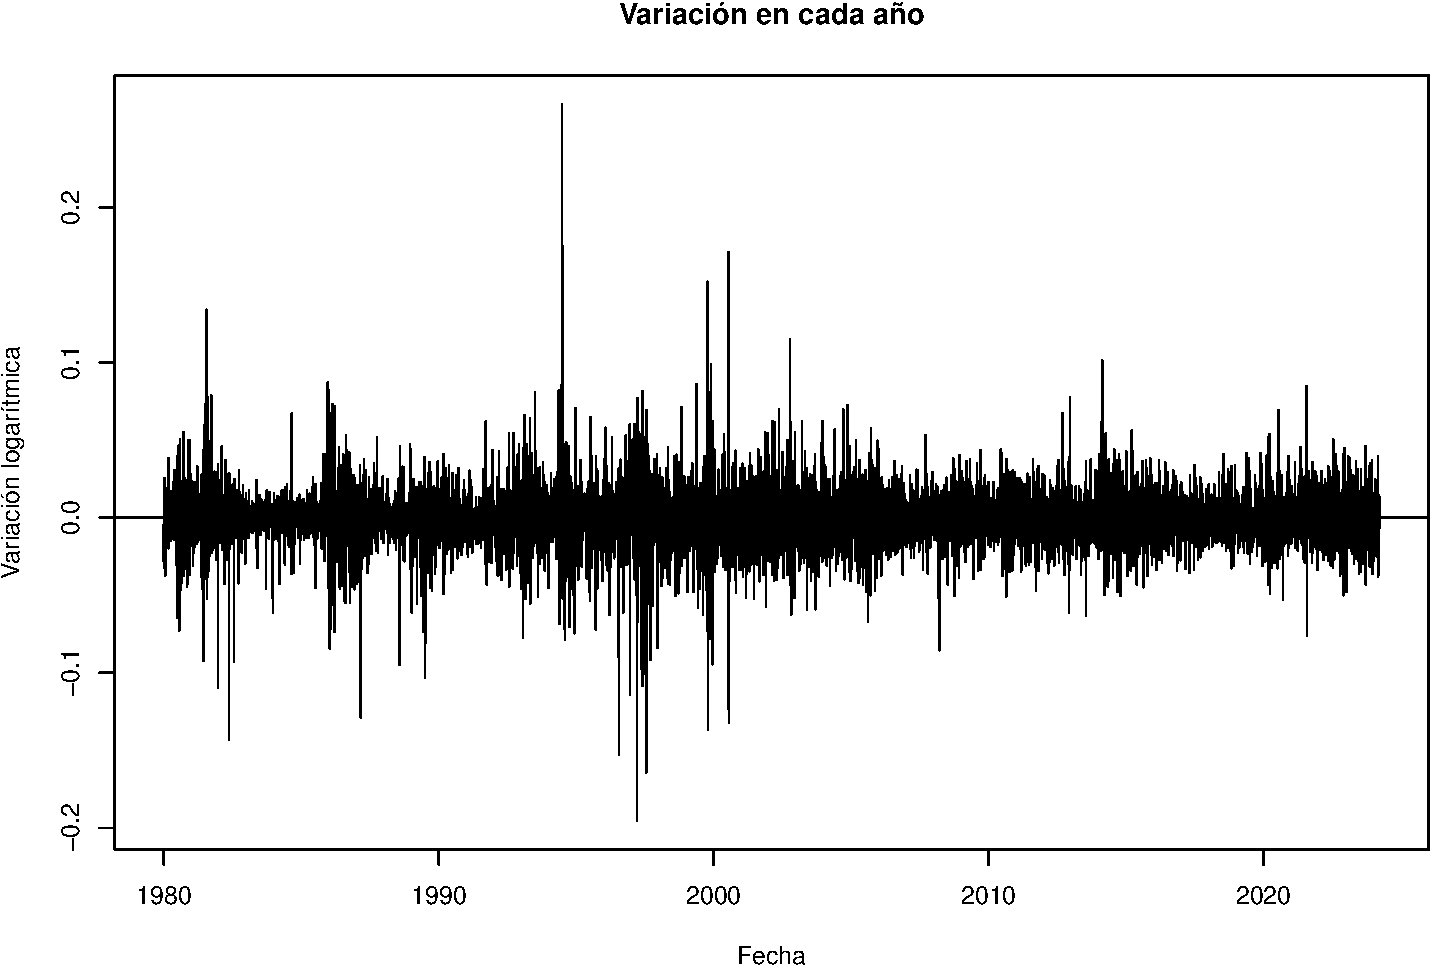
\includegraphics{Informe_files/figure-beamer/unnamed-chunk-8-1.pdf}
\end{frame}

\begin{frame}[fragile]{}
\phantomsection\label{section-3}
\begin{Shaded}
\begin{Highlighting}[]
\FunctionTok{plot}\NormalTok{(decomposition\_2000}\SpecialCharTok{$}\NormalTok{seasonal, }
     \AttributeTok{ylab =} \StringTok{"Estacionalidad"}\NormalTok{, }\AttributeTok{xlab =} \StringTok{""}\NormalTok{)}
\end{Highlighting}
\end{Shaded}

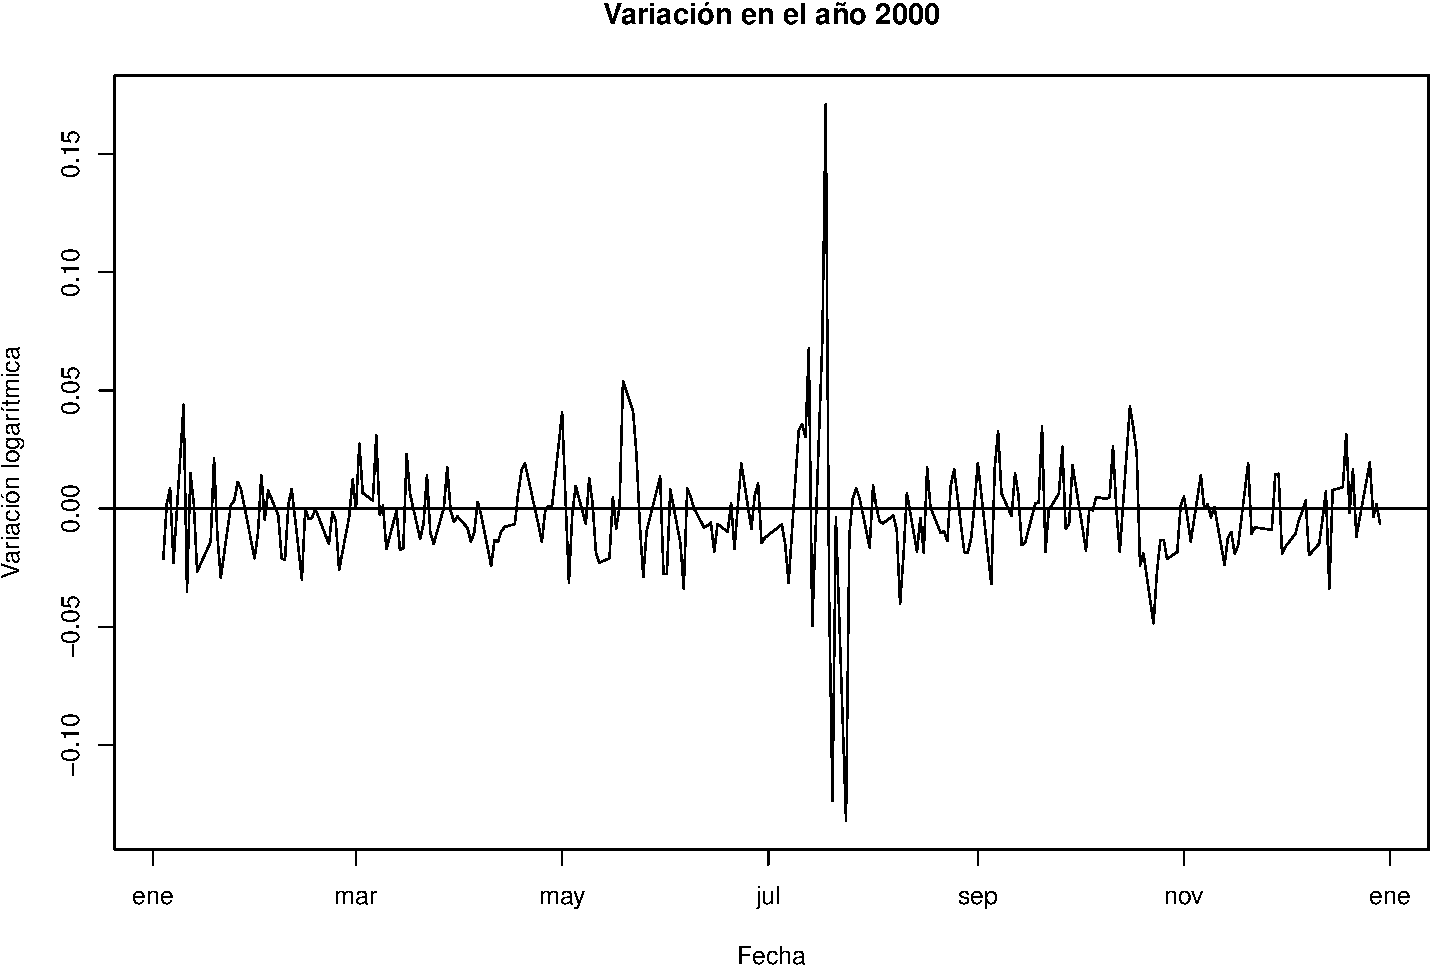
\includegraphics{Informe_files/figure-beamer/unnamed-chunk-9-1.pdf}
\end{frame}

\begin{frame}[fragile]{}
\phantomsection\label{section-4}
\begin{Shaded}
\begin{Highlighting}[]
\FunctionTok{plot}\NormalTok{(decomposition\_2000}\SpecialCharTok{$}\NormalTok{random, }
     \AttributeTok{ylab =} \StringTok{"Residuales"}\NormalTok{, }\AttributeTok{xlab =} \StringTok{""}\NormalTok{)}
\end{Highlighting}
\end{Shaded}

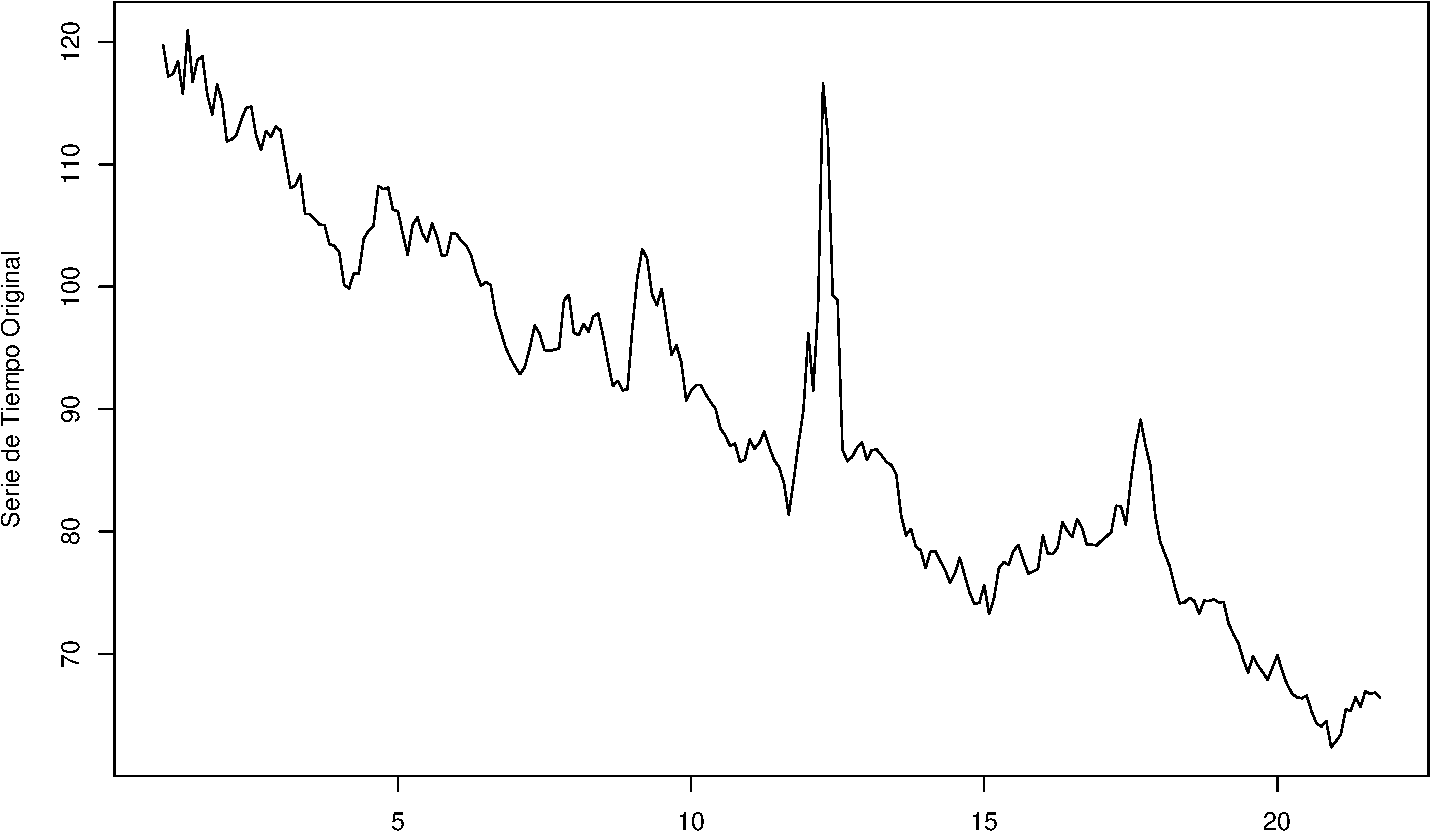
\includegraphics{Informe_files/figure-beamer/unnamed-chunk-10-1.pdf}
\end{frame}

\begin{frame}[fragile]{Análisis de tendencia}
\phantomsection\label{anuxe1lisis-de-tendencia}
\begin{Shaded}
\begin{Highlighting}[]
\FunctionTok{plot}\NormalTok{(decomposition\_2000}\SpecialCharTok{$}\NormalTok{x, }
     \AttributeTok{ylab =} \StringTok{"Serie de Tiempo Original"}\NormalTok{, }\AttributeTok{xlab =} \StringTok{""}\NormalTok{)}
\FunctionTok{abline}\NormalTok{(}\FunctionTok{lm}\NormalTok{(decomposition\_2000}\SpecialCharTok{$}\NormalTok{x }
          \SpecialCharTok{\textasciitilde{}} \FunctionTok{time}\NormalTok{(decomposition\_2000}\SpecialCharTok{$}\NormalTok{x)), }\AttributeTok{col =} \StringTok{"red"}\NormalTok{)}
\end{Highlighting}
\end{Shaded}

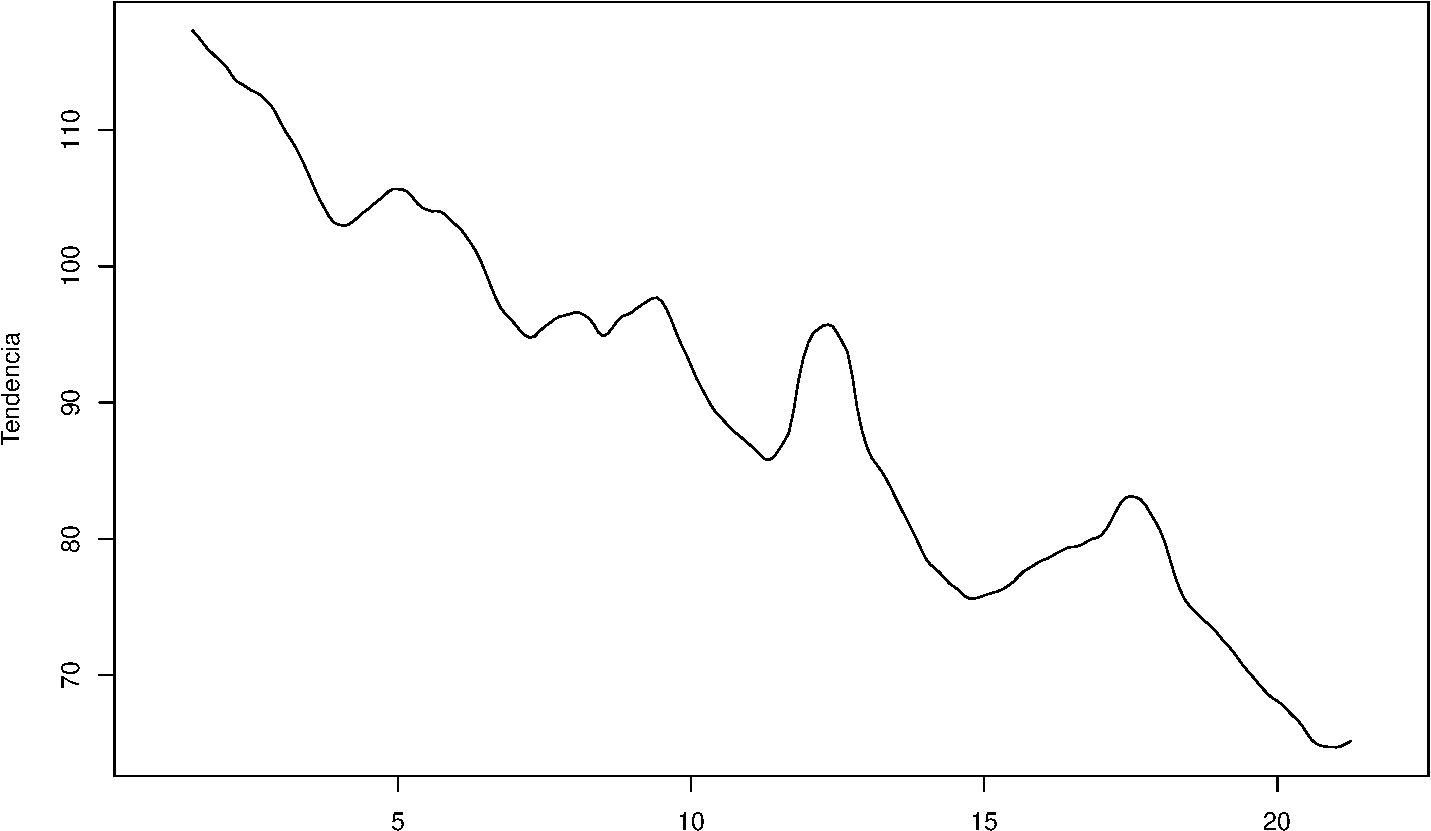
\includegraphics{Informe_files/figure-beamer/unnamed-chunk-11-1.pdf}
\end{frame}

\begin{frame}[fragile]{}
\phantomsection\label{section-5}
\begin{Shaded}
\begin{Highlighting}[]
\FunctionTok{plot}\NormalTok{(decomposition\_2000}\SpecialCharTok{$}\NormalTok{trend, }
     \AttributeTok{ylab =} \StringTok{"Tendencia"}\NormalTok{, }\AttributeTok{xlab =} \StringTok{""}\NormalTok{)}
\end{Highlighting}
\end{Shaded}

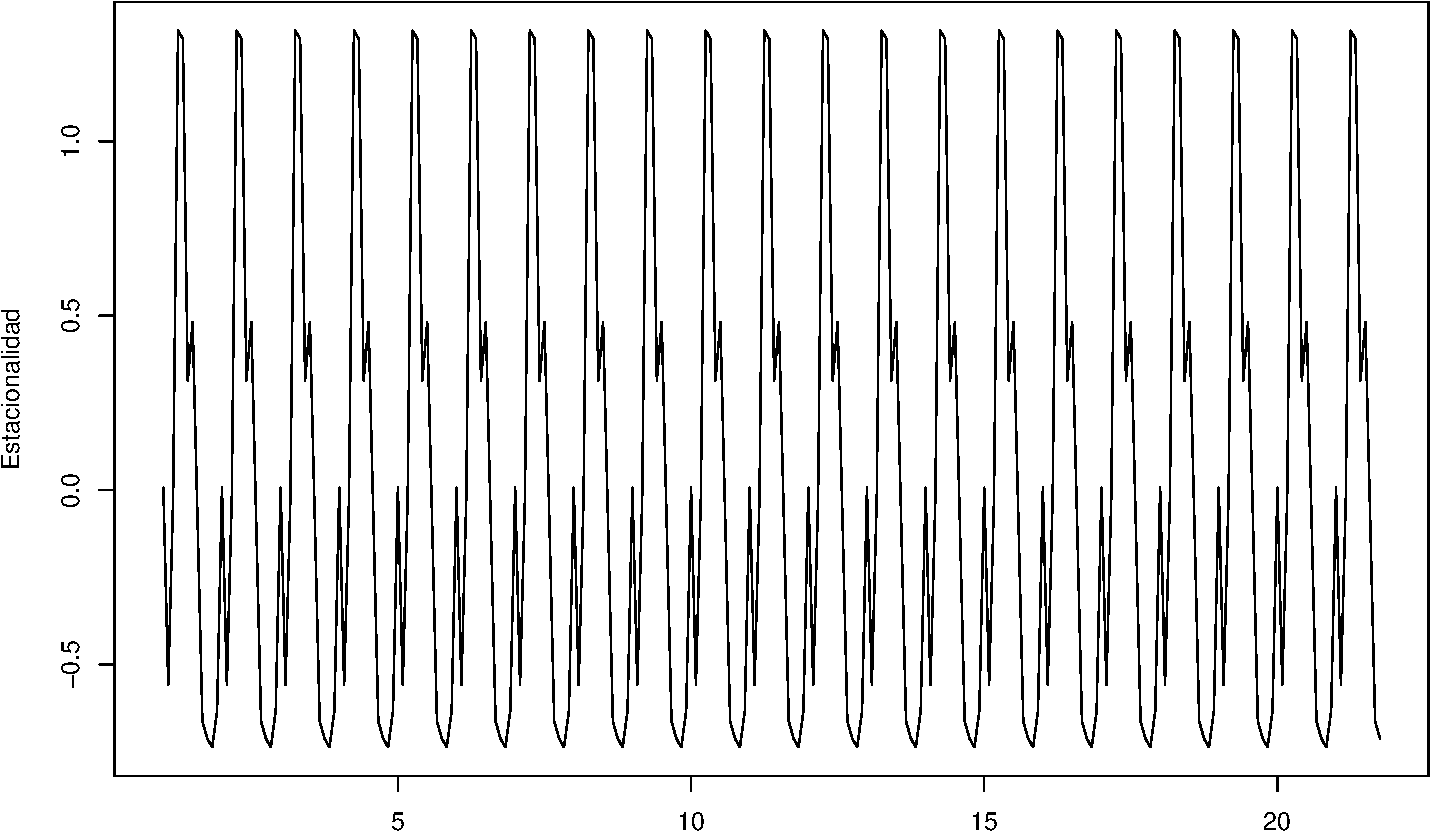
\includegraphics{Informe_files/figure-beamer/unnamed-chunk-12-1.pdf}
\end{frame}

\begin{frame}[fragile]{Estacionariedad}
\phantomsection\label{estacionariedad}
\[H_0: \text{no es estacionaria.}\] \[H_1: \text{Es estacionaria}\]

\begin{Shaded}
\begin{Highlighting}[]
\CommentTok{\#install.packages("urca")}
\FunctionTok{library}\NormalTok{(urca)}
\NormalTok{adf\_test }\OtherTok{\textless{}{-}} \FunctionTok{ur.df}\NormalTok{(KCN4\_2000, }\AttributeTok{type =} \StringTok{"trend"}\NormalTok{, }\AttributeTok{lags =} \DecValTok{1}\NormalTok{)}
\NormalTok{summary\_text }\OtherTok{\textless{}{-}} \FunctionTok{capture.output}\NormalTok{(}\FunctionTok{summary}\NormalTok{(adf\_test))}
\NormalTok{tail\_summary }\OtherTok{\textless{}{-}} \FunctionTok{tail}\NormalTok{(summary\_text, }\AttributeTok{n =} \DecValTok{11}\NormalTok{)}
\NormalTok{tail\_summary\_df }\OtherTok{\textless{}{-}} \FunctionTok{data.frame}\NormalTok{(tail\_summary)}
\FunctionTok{colnames}\NormalTok{(tail\_summary\_df) }\OtherTok{\textless{}{-}} \FunctionTok{c}\NormalTok{(}\StringTok{"Resumen"}\NormalTok{)}
\end{Highlighting}
\end{Shaded}
\end{frame}

\begin{frame}[fragile]{}
\phantomsection\label{section-6}
\begin{Shaded}
\begin{Highlighting}[]
\NormalTok{tail\_summary\_df}
\end{Highlighting}
\end{Shaded}

\begin{verbatim}
##                                                    Resumen
## 1  F-statistic: 8.203 on 3 and 244 DF,  p-value: 3.185e-05
## 2                                                         
## 3                                                         
## 4      Value of test-statistic is: -4.6517 7.7753 10.8352 
## 5                                                         
## 6                    Critical values for test statistics: 
## 7                                         1pct  5pct 10pct
## 8                                   tau3 -3.99 -3.43 -3.13
## 9                                   phi2  6.22  4.75  4.07
## 10                                  phi3  8.43  6.49  5.47
## 11
\end{verbatim}
\end{frame}

\begin{frame}{Conclusión}
\phantomsection\label{conclusiuxf3n}
En este informe, se han analizado y visualizado los precios del café a
lo largo del tiempo utilizando técnicas de análisis descriptivo. Se han
identificado tendencias y patrones en los datos, y se han aplicado
técnicas de estabilización de la v arianza y descomposición de la serie
de tiempo. Además, se ha calculado y graficado la autocorrelación para
cada año.
\end{frame}

\end{document}
